\section{Experiment A: what the in-context predictor computes}\label{sec:expa}

\begin{figure}[t]
\centering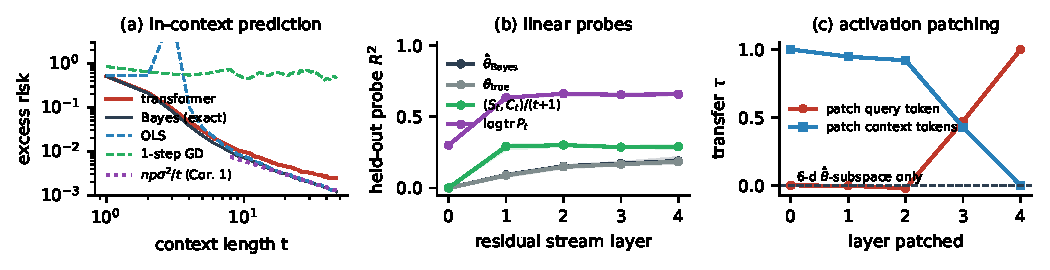
\includegraphics[width=\linewidth]{figs/fig_a.pdf}
\vspace{-6mm}
\caption{\textbf{A, pre-registered analyses} (3 seeds). (a)~Excess risk vs.\ context length. The transformer tracks the
exact Bayes predictor while data are scarce, then flattens at an approximation floor. The Bayes curve follows the
parameter-free law of Cor.~\ref{cor:law}. (b)~Held-out linear probes of the residual stream (band: range over
seeds). The estimate $\hat\theta_t$ is barely decodable; the posterior uncertainty is. (c)~Activation patching of
episode $A$ into $B$. Patching the query token transfers $A$'s behaviour only from layer~3 on. Patching the 6-d
$\hat\theta$-probe subspace transfers nothing (dashed).}
\label{fig:a}
\vspace{-3mm}
\end{figure}

\paragraph{Behaviour: Bayes-optimal while data are scarce, then an approximation floor.} The trained predictor is
much closer to the exact Bayes predictor than to OLS or to one GD step. The mean algorithmic distance to OLS exceeds
the distance to Bayes by \AdOLS\ \AdOLSci, and the distance to GD exceeds it by \AdGD\ \AdGDci\ (H1a, H1b; Holm $p\PHonea$,
$\PHoneb$). For $t\le4$ its excess risk is within a factor \Ashort\ of Bayes. After that it decays more slowly than $1/t$ and
settles about $\Afloor\times10^{-3}$ above Bayes. Meanwhile $t\,\mathcal{R}^\star_t$ reaches \AtBayes\ at $t{=}47$:
Theorem~\ref{thm:bayes} gives \AtTheory\ and Corollary~\ref{cor:law} predicts $np\sigma^2{=}0.06$. The pre-registered
tolerance H1c is \textbf{rejected}: the mean excess ratio is \Aratio\ \Aratioci, against a threshold of $1.25$. This is
the dynamical analogue of the observation that trained transformers fall short of least-squares
rates~\citep{hill2025transformers,cole2025incontext}. Longer training and larger models narrow the gap but do not
close it (\S\ref{sec:scale}).

\paragraph{The pre-registered mechanism is rejected: no estimate in the residual stream.} The best linear probe of
the residual stream for $\hat\theta_t$ reaches only $R^2{=}\ARtheta$ \ARthetaci\ (H2a, threshold $0.8$:
rejected). It beats the probe for the true $\theta$ by just \AdR\ (H2b: significant but negligible). The normalised
sufficient statistics are partly decodable ($R^2{\le}\Amom$) and peak at layers 1--2, before $\hat\theta$ peaks at
layer~4, in every seed. So H2c holds formally but is uninformative. What \emph{is} linearly decodable is the
model's uncertainty: $\log\operatorname{tr}P_t$ reaches $R^2{=}\Alogtr$. Steering along the $\hat\theta$-probe
directions does not move the prediction (slope \Aslope; H3a rejected). Swapping the 6-d probe subspace of the query
between episodes transfers $\tau{=}\Atausub$ of the behaviour, which is less than a random 6-d subspace (\Ataurand; H3b
rejected). Whole-stream patching (Fig.~\ref{fig:a}c) shows that parameter information enters the query position
only in blocks 3--4: $\tau_{\rm last}{=}\AtauLastThree$ after block~3, while patching all context positions at
layer~2 still transfers $\ge\AtauCtxTwo$.

\begin{figure}[t]
\centering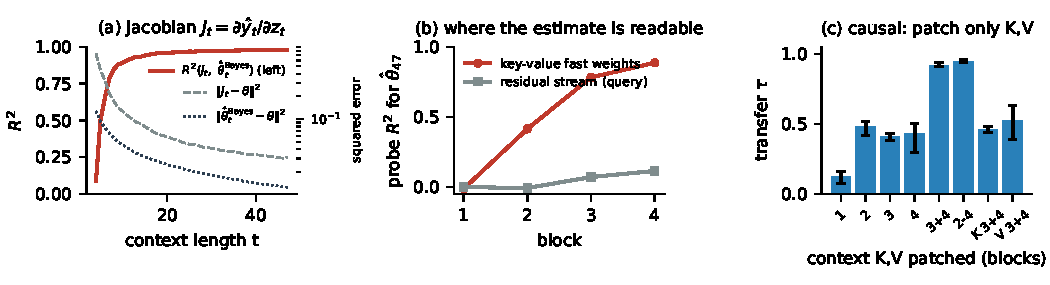
\includegraphics[width=\linewidth]{figs/fig_mech.pdf}
\vspace{-6mm}
\caption{\textbf{A, exploratory follow-up: where the estimate lives} (3 seeds). (a)~The predictor's Jacobian with
respect to its query, $J_t{=}\partial\hat y_t/\partial z_t$, matches the Bayes estimate. Its error to the truth
(dashed) tracks the Bayes estimate's error (dotted). (b)~$\hat\theta_{47}$ is linearly readable from the per-block
key--value fast weights $\widehat{\mathrm{Cov}}(v,k)$ but not from the residual stream at the same position.
(c)~Patching \emph{only} the context keys and values of blocks 3--4, leaving every activation of the query untouched,
transfers over 90\% of the other episode's behaviour. Keys or values alone transfer about half.}
\label{fig:mech}
\vspace{-3mm}
\end{figure}

\paragraph{Exploratory: the estimate lives in the keys and values, and acts through the query Jacobian.} The
following analyses were added after the pre-registered ones failed, and they are labelled as such. Remark~\ref{rem:fw}
suggests where to look.
\begin{itemize}
\item \emph{The answer is linearly represented; the parameter is not.} A linear probe recovers the Bayes
\emph{prediction} $\hat\theta_tz_t$ with $R^2{=}\AyhatLthree$ after block~3 and $\AyhatLfour$ after block~4. An MLP probe
recovers $\hat\theta_t$ itself only up to $R^2{=}\AmlpTheta$.
\item \emph{The Jacobian is the estimate.} The predictor is close to linear in its own query: counterfactual queries are explained with
$R^2{=}\AcfLin$ by its Jacobian, and their effect has slope \AcfSlope\ against the Bayes map. Its Jacobian
$J_t{=}\partial\hat y_t/\partial z_t$ matches $\hat\theta^{\rm Bayes}_t$ with $R^2{=}\AjacBayes$, more closely than it
matches the truth ($\AjacTrue$) or OLS ($\AjacOLS$) (Fig.~\ref{fig:mech}a).
\item \emph{It is stored in key--value memory.} The per-head fast weights $\widehat{\mathrm{Cov}}(v,k)$ of
block~4 predict $\hat\theta_{47}$ with $R^2{=}\AfwR$ (block 3: \AfwRthree). The residual stream at the same position
gives at most \AresidR\ (Fig.~\ref{fig:mech}b).
\item \emph{The memory is causal.} Replacing only the context keys and values of blocks 3--4 by those of another episode,
with the query's residual stream, its attention queries and all MLPs left as they were, transfers $\tau{=}\AkvThreeFour$ of that
episode's behaviour (blocks 2--4: \AkvTwoFour). Keys alone give \AkOnly\ and values alone \AvOnly
(Fig.~\ref{fig:mech}c). The carriers are 2--3 heads per block with near-uniform attention, as in Remark~\ref{rem:fw}.
\item \emph{Probe directions are not the model's directions.} Even for the well-decoded prediction, steering along the
probe direction has slope only \AsteerYhat, and swapping the probe subspace transfers only \AtauYhat. Linear decodability did not imply
causal use anywhere in this study.
\end{itemize}
In short, the transformer does implement near-Bayes system identification. It does not do so by writing $\hat\theta$
into an activation. The estimate is spread over the key--value memory of the context and is read out, applied to the query, by
attention. This is why RMA-style ``latent parameter'' probes of the residual stream~\citep{kumar2021rma,chamachot2026evaluating}
can fail even when adaptation works.

\section{Experiment B: nonlinear and contact physics in MuJoCo}\label{sec:expb}

\begin{figure}[t]
\centering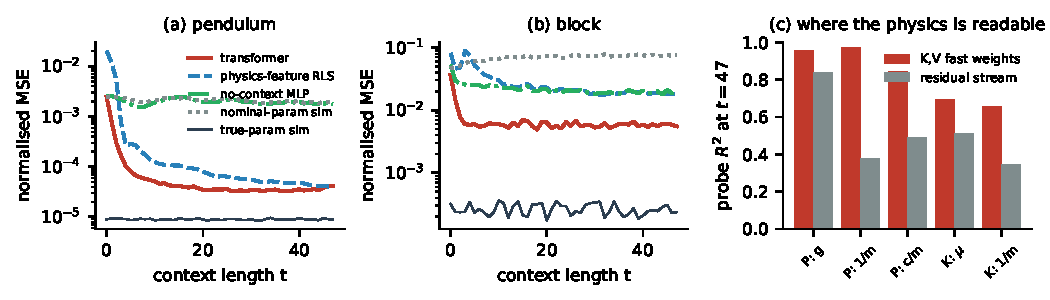
\includegraphics[width=\linewidth]{figs/fig_b.pdf}
\vspace{-6mm}
\caption{\textbf{B} (3 seeds). (a, b)~Normalised one-step error vs.\ context length. On the pendulum the transformer
beats physics-feature RLS, even though RLS has the true model class up to discretisation. On the stick--slip block it beats RLS by $3\times$. (c)~Residual-stream probes
(fixed final-position probe applied at every $t$).}
\label{fig:b}
\vspace{-3mm}
\end{figure}

\paragraph{Prediction.} Averaged over $t{=}24..47$, the normalised error on the pushed block with Coulomb friction is
\BKTF\ for the transformer and \BKRLS\ for physics-feature RLS (H4a: difference \HfourA\ \HfourAci, Holm $p\PHfoura$).
For comparison, the no-context MLP gets \BKMLP, nominal-parameter simulation \BKNom, and simulation with the true parameters
\BKOrc. On the pendulum, where feature RLS has the right model class up to discretisation, the transformer
(\BPTF) still beats it (\BPRLS). Nominal simulation (\BPNom) and the no-context MLP (\BPMLP) are $\sim$60$\times$ worse,
so the gain comes from in-context adaptation.

\paragraph{Mechanism.} The pre-registered probes again fail for the parameters that enter the dynamics
multiplicatively. Residual-stream $R^2$ at $t{=}47$ is \BprobePg\ for $g$, \BprobePinvm\ for $1/m$ and \BprobeKmu\ for
$\mu$ (H4c rejected). Steering along the $1/m$ probe moves the input sensitivity the right way in only
\BsteerP\% (pendulum) and \BsteerK\% (block) of episodes (H4d rejected). The exploratory analyses of \S\ref{sec:expa}
transfer. The model's own sensitivity $\partial\dot q_{t+1}/\partial u_t$, its functional estimate of $1/m$, correlates
with the true $1/m$ at $r{=}\BfuncP$ on the pendulum; on the block it is $r{=}\BfuncK$, because the sensitivity is zero while stuck. The
key--value fast weights decode $1/m$ with $R^2{=}\BfwPinvm$ (residual: \BresPinvm), and on the block they decode $\mu$ at \BfwKmu\ (residual
\BresKmu). \PENDING{bouncer}

\section{Experiment C: does an in-context controller explore?}\label{sec:expc}
\PENDING{resC}

\section{Scale and training length}\label{sec:scale}
\PENDING{resScale}

\section{Discussion and limitations}\label{sec:disc}
\PENDING{discussion}
